\begin{figure}[h!]
  \begin{minipage}[c]{0.48\textwidth}
    \caption{
      \textbf{The smoothing approach is expected to be more robust than the bin approach.} Both panels depict the same mutation location data for a hypothetical chromosome, with the black dots below the x-axis representing the true location of mutations. By binning the genome by convention, one counts the number of mutations in each yellow bin. The obtained GLE data is then the yellow dots on top of each bin. This binned GLE data changes when shifting the bin boundaries from panel (a) to panel (b). On the contrary, the smooth representation of GLE, which adopts \gls{density} estimation, is depicted by the blue dots on the blue line. By smoothing the genome, GLE data is the same for both panels. 
    } \label{fig:mutdistribution_demo}
  \end{minipage}\hfill
  \begin{minipage}[c]{0.55\textwidth}
    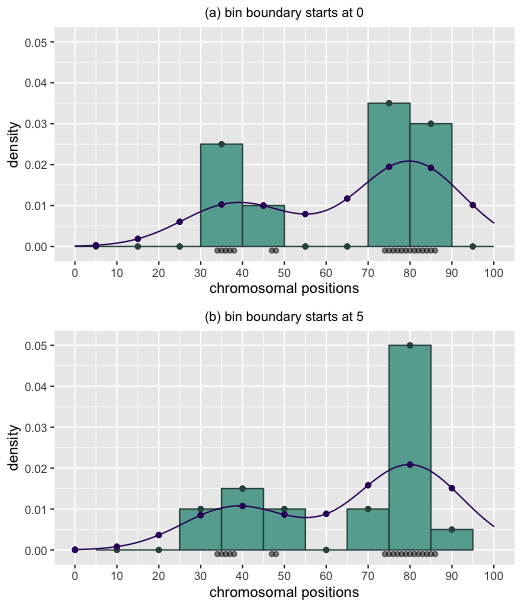
\includegraphics[width=\textwidth]{graphics/mutdistribution_demo.png}
  \end{minipage}
\end{figure}
